% $Header: /cvsroot/latex-beamer/latex-beamer/solutions/conference-talks/conference-ornate-20min.en.tex,v 1.6 2004/10/07 20:53:08 tantau Exp $

\documentclass[usenames,dvipsnames]{beamer}

\mode<presentation>
{
%  \usetheme{Hannover}
\usetheme[width=0.7in]{Hannover}
% or ...

  \setbeamercovered{transparent}
  % or whatever (possibly just delete it)
}
\usepackage{longtable}
\usepackage{booktabs}
\usepackage{bnf}
\usepackage{bm}

%\usepackage{qtree}

\usepackage[english]{babel}
% or whatever

\usepackage[latin1]{inputenc}
% or whatever

\usepackage{times}
%\usepackage[T1]{fontenc}
% Or whatever. Note that the encoding and the font should match. If T1
% does not look nice, try deleting the line with the fontenc.
%\usepackage{logictheme}

\usepackage{multirow}
\usepackage{totpages}
\usepackage{hyperref}
\usepackage{booktabs}
\usepackage[round]{natbib}

\usepackage{listings}
% \lstset{frame=none, showstringspaces=false, basicstyle=\ttfamily\footnotesize,
%   xleftmargin=-8mm,language=Haskell}
\lstset{frame=none, showstringspaces=false, basicstyle=\ttfamily\bfseries\footnotesize,
  xleftmargin=-8mm,language=Haskell,breaklines=true}

\usepackage{tikz}
\usetikzlibrary{positioning}

\hypersetup{colorlinks=true,
    linkcolor=blue,
    citecolor=blue,
    filecolor=blue,
    urlcolor=blue,
    unicode=false}

\usepackage{pifont}
\usepackage{amsmath, amsfonts, amssymb, xspace, xcolor, url}
\newcommand{\cross}{{\LARGE {\color{red}\ding{55}}}}

\newcommand{\greencheck}{{\LARGE {\color{ForestGreen}\checkmark}}}
\newcommand{\bluedash}{{\LARGE {\color{blue}{--}}}}

\newcommand{\blt}{- } %used for bullets in a list

\newcounter{datadefnum} %Datadefinition Number
\newcommand{\ddthedatadefnum}{DD\thedatadefnum}
\newcommand{\ddref}[1]{DD\ref{#1}}

\newcommand{\colAwidth}{0.1\textwidth}
\newcommand{\colBwidth}{0.8\textwidth}

\renewcommand{\arraystretch}{1.1} %so that tables with equations do not look crowded

\newcounter{rqnum} %research question number
\newcommand{\rqtherqnum}{RQ`'\therqnum}
\newcommand{\rqref}[1]{RQ\ref{#1}}

\pgfdeclareimage[height=0.7cm]{logo}{McMasterLogo}
\title[\pgfuseimage{logo}] % (optional, use only with long paper titles)
{Digging Deeper Into the State of the Practice for Domain Specific Research Software}

%\subtitle
%{Include Only If Paper Has a Subtitle}

\author[Slide \thepage~of \pageref{TotPages}] % (optional, use only with lots of
                                              % authors)
{\textbf{Spencer Smith}, Peter Michalski}
% - Give the names in the same order as the appear in the paper.
% - Use the \inst{?} command only if the authors have different
%   affiliation.

\institute[McMaster University] % (optional, but mostly needed)
{
  Computing and Software Department\\
  Faculty of Engineering\\
  McMaster University
}
% - Use the \inst command only if there are several affiliations.
% - Keep it simple, no one is interested in your street address.

\date[June 23, 2022] % (optional, should be abbreviation of conference name)
{ICCS SE4Science, June 23, 2022}
% - Either use conference name or its abbreviation.
% - Not really informative to the audience, more for people (including
%   yourself) who are reading the slides online

\subject{research software, software engineering, empirical measurement}
% This is only inserted into the PDF information catalog. Can be left
% out. 

% If you have a file called "university-logo-filename.xxx", where xxx
% is a graphic format that can be processed by latex or pdflatex,
% resp., then you can add a logo as follows:

%\pgfdeclareimage[height=0.5cm]{Mac-logo}{McMasterLogo}
%\logo{\pgfuseimage{Mac-logo}}

% Delete this, if you do not want the table of contents to pop up at
% the beginning of each subsection:
% \AtBeginSubsection[]
% {
%   \begin{frame}<beamer>
%     \frametitle{Outline}
%     \tableofcontents[currentsection,currentsubsection]
%   \end{frame}
% }

% If you wish to uncover everything in a step-wise fashion, uncomment
% the following command: 

%\beamerdefaultoverlayspecification{<+->}

\beamertemplatenavigationsymbolsempty 

% have SRS and LP open during the presentation

\begin{document}

%%%%%%%%%%%%%%%%%%%%%%%%%%%%%%%%%%%%%%
\hoffset=-.4in %removing side bar for these frames
\begin{frame}[plain]

\begin{tikzpicture}[remember picture,overlay]
  \node [xshift=1.3cm,yshift=0cm] at (current page.center)
  {
  \includegraphics[width=1.5\textwidth]{diggingspringsoil.jpeg}
  };
\end{tikzpicture}

\titlepage

\end{frame}
\hoffset=0in %restore
%%%%%%%%%%%%%%%%%%%%%%%%%%%%%%%%%%%%%%

% \begin{frame}

% \frametitle{Literate Scientific Software}
% \tableofcontents
% % You might wish to add the option [pausesections]

% % make like a story - the phases - reason for, why works, advantages
% % changing the history a bit to make a more rational narrative

% \end{frame}

%%%%%%%%%%%%%%%%%%%%%%%%%%%%%%%%%%%%%%

\begin{frame}

\frametitle{Outline}

\begin{itemize}
  \item Motivation and Example
  %\item Research Questions (RQs)
  \item Overview of SOP Assessment Methodology
  \item Identify Software (RQ1)
  \item Rank
  \begin{itemize}
  \item By Best Practices (RQ2)
  \item Versus Community Ranking (RQ3)
  \end{itemize}
  \item Comparison to Other Research Software
  \begin{itemize}
  \item Artifacts (RQ4)
  \item Tools (RQ5)
  \item Processes (RQ6)
  \item Pain Points (RQ7, RQ8)
  \end{itemize}
  \item Threats to Validity
  \item Concluding Remarks
\end{itemize}

% \begin{tikzpicture}[remember picture,overlay]
%   \node [xshift=3.4cm,yshift=-2.0cm] at (current page.center)
%   {
%   \includegraphics[width=0.47\textwidth]{backpain.jpeg}
%   };
% \end{tikzpicture}
  
\end{frame}

%%%%%%%%%%%%%%%%%%%%%%%%%%%%%%%%%%%%%%

\section[Motivation]{Motivation and Running Example}

%%%%%%%%%%%%%%%%%%%%%%%%%%%%%%%%%%%%%%

\begin{frame}

\frametitle{Motivation}

\begin{itemize}
%\item Understand research soft dev to improve. %including productivity, sustainability etc.
\item Previous studies:
\begin{itemize}
\item Survey developers \citep{HannayEtAl2009, Nguyen-HoanEtAl2010,
PintoEtAl2018}.
\item Mining \citep{GrannanEtAl2020, SoodEtAl2019}.
\item Recruit broadly, or by prog lang \citep{PintoEtAl2018}, or role of developer \citep{UditAndKatz2017}.
\item Case studies \citep{CarverEtAl2007,Segal2005}.
\end{itemize}
\item We focus on:
\begin{itemize}
  \item Contents of repositories (manual and automated),
  \item Interviews with developers,
  \item One domain at a time.
\end{itemize}
\item Include Domain Expert in the assessment.
\item Help users select software.
\item Learn what works in a domain, and what doesn't.
%\item Better response to customized feedback.
%\item Future meta-analysis.
\end{itemize}

\end{frame}

%%%%%%%%%%%%%%%%%%%%%%%%%%%%%%%%%%%%%%

\hoffset=-.4in %removing side bar for these frames
\begin{frame}[plain]

\frametitle{LBM Running Example}

\begin{tikzpicture}[remember picture, overlay]
  \node [xshift=1.0cm,yshift=0.0cm] at (current page.center)
  {
  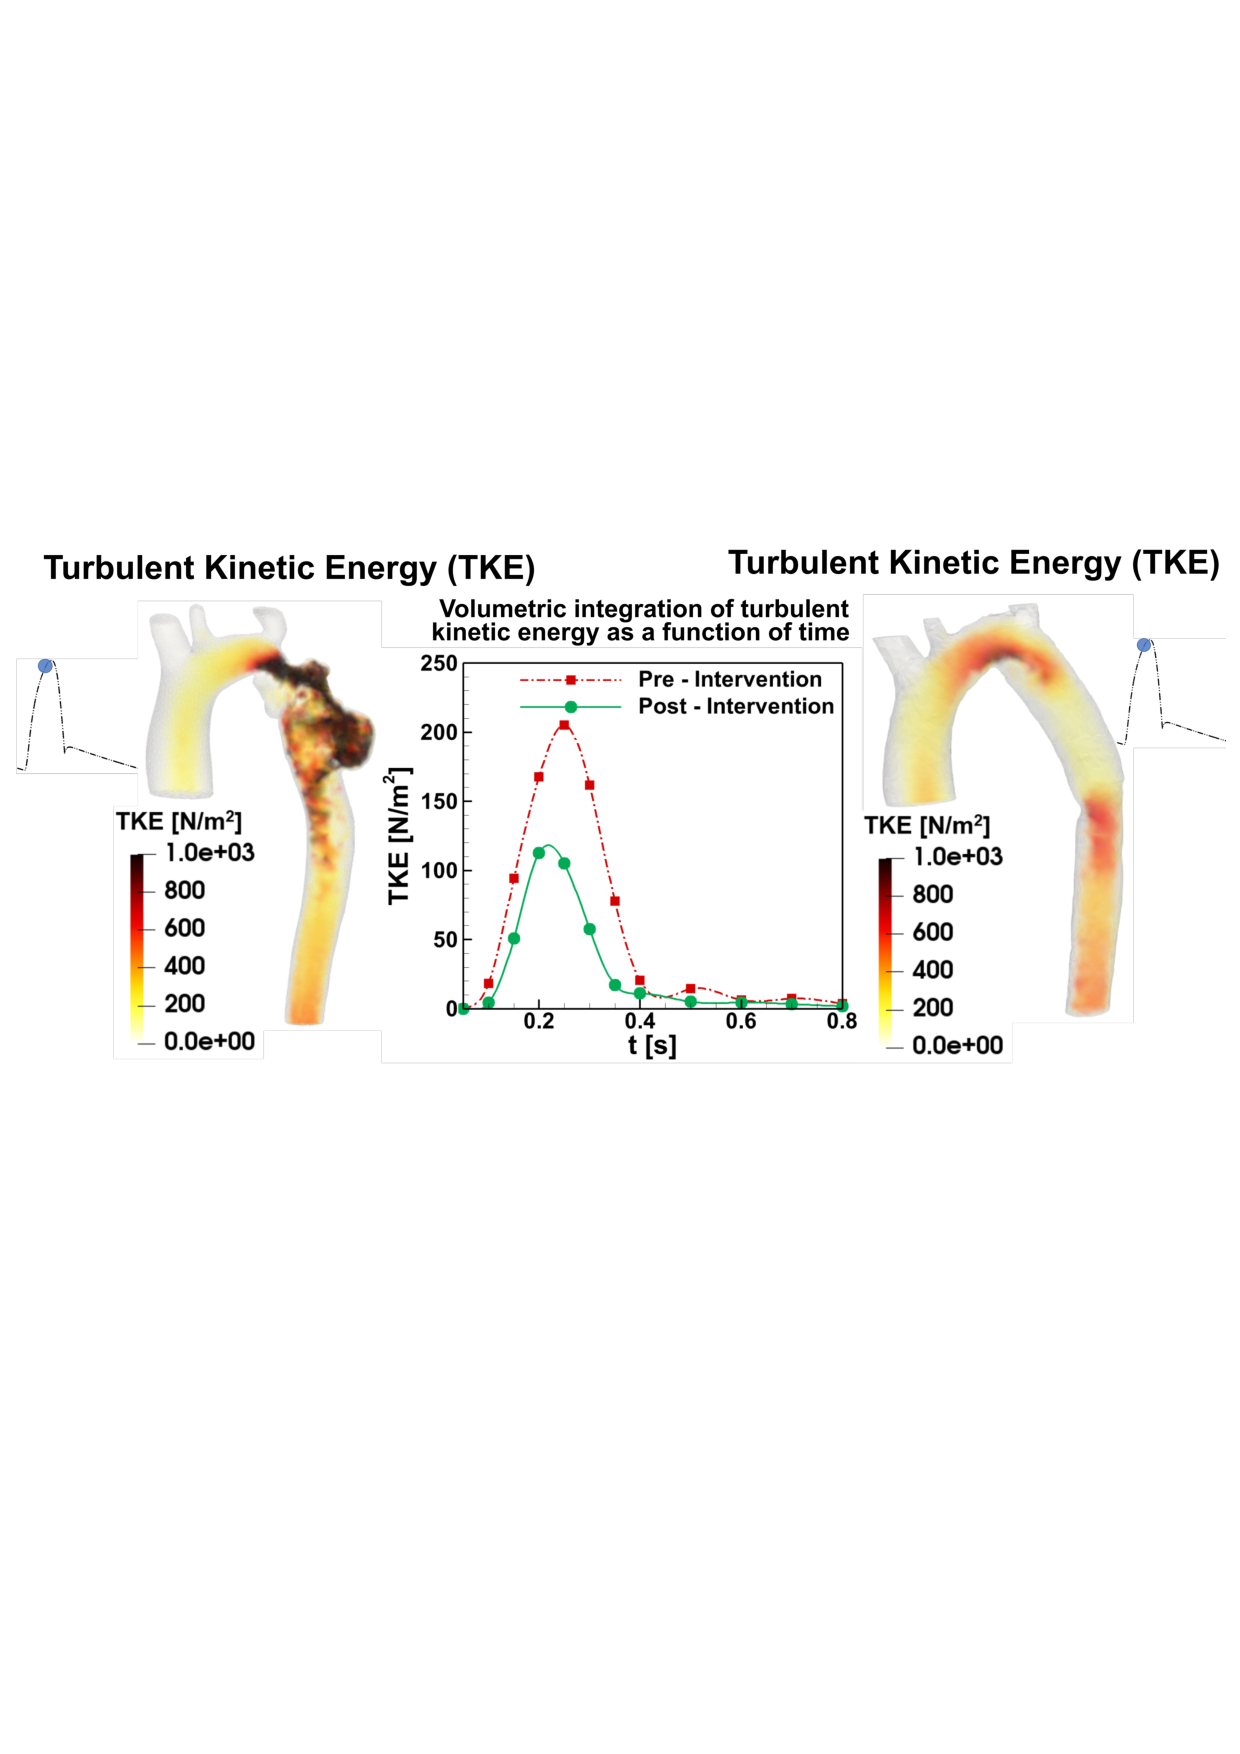
\includegraphics[width=1.2\textwidth]{../figures/LBMExample.pdf}
  };
\end{tikzpicture}
  
\end{frame}
\hoffset=0in %restore

%%%%%%%%%%%%%%%%%%%%%%%%%%%%%%%%%%%%%%
  
% \section[RQs]{Research Questions}

% %%%%%%%%%%%%%%%%%%%%%%%%%%%%%%%%%%%%%%

% \begin{frame}

%   \frametitle{Research Questions}

%   \begin{enumerate}
%     \item[RQ\refstepcounter{rqnum}\therqnum \label{RQ_WhatProjects}:] What
%     software projects exist in the domain%, with the constraint that the source
%     %code must be available for all identified projects?
%     \item [RQ\refstepcounter{rqnum}\therqnum \label{RQ_HighestQuality}:] Which
%     of the projects identified in \rqref{RQ_WhatProjects} follow current best
%     practices %, based on evidence found by experimenting with the software and
%     %searching the artifacts available in each project's repository? %define
%     %best practices
%     \item [RQ\refstepcounter{rqnum}\therqnum \label{RQ_CompareHQ2Popular}:] How
%     does \rqref{RQ_HighestQuality} compare to community ranking?
%     \item [RQ\refstepcounter{rqnum}\therqnum \label{RQ_CompareArtifacts}:] How
% 	  do domain artifacts compare to research software in general?
% 	  \item [RQ\refstepcounter{rqnum}\therqnum \label{RQ_CompareToolsProjMngmnt}:]
% 	  How do domain tools compare to research software in general?
% 	  \item [RQ\refstepcounter{rqnum}\therqnum \label{RQ_CompareMethodologies}:]
% 	  How do domain processes compare to research software in general?
%     \item [RQ\refstepcounter{rqnum}\therqnum \label{RQ_PainPoints}:] What are
%     the pain points for developers?
%     \item [RQ\refstepcounter{rqnum}\therqnum \label{RQ_ComparePainPoints}:] How
%     do the pain points compare to research software in general?
  
%   \end{enumerate}
    
% \end{frame}
  
% %%%%%%%%%%%%%%%%%%%%%%%%%%%%%%%%%%%%%%

\section[Methodology]{Overview of SOP Assessment Methodology}

%%%%%%%%%%%%%%%%%%%%%%%%%%%%%%%%%%%%%%

\begin{frame}

  \frametitle{Methodology}
  
  From \citet{SmithEtAl2021}:

  \begin{enumerate}
    \item Identify the domain of interest.
    \item List candidate software packages for the domain.
    \item Filter the software package list.
    %\item Gather the source code and documentation for each software package.
    \item Measure using the measurement template.
    \begin{itemize}
      \item 10 qualities (installability, correctness, reliability, etc.).
      \item 108 measures.
    \end{itemize}
    \item Use AHP to rank the software packages.
    \item Interview the developers (Semi-structured).
    \begin{itemize}
      \item 20 questions.
      \item How they organize their projects?
      \item Their understanding of the users?
      \item Current and past difficulties?
      \item Solutions the team has found or will try?
      \item Use of documentation?
    \end{itemize}
    \item Domain analysis.
    %\item Answer research questions.
  \end{enumerate}
  
\end{frame}
  
%%%%%%%%%%%%%%%%%%%%%%%%%%%%%%%%%%%%%%

\begin{frame}

  \frametitle{Identify Software (RQ1)}

  Chosen domain should have the following properties:

  \begin{enumerate}
  \item Well-defined and stable theoretical underpinnings.
  \item A community of people studying it.
  \item Open source options.
  \item Approximately 30 candidate packages.
  \end{enumerate}	
  
  Find candidates via:
  
  \begin{enumerate}
    \item Search engine queries.
    \item \href{https://github.com/} {GitHub}.
    \item \href{https://swmath.org/} {swMATH}.
    \item Scholarly articles.
    \item Domain Expert.
  \end{enumerate}

\end{frame}

%%%%%%%%%%%%%%%%%%%%%%%%%%%%%%%%%%%%%%

\hoffset=-.82in %removing side bar for these frames
\begin{frame}[plain]

%\frametitle{Domain Analysis}
  \begin{tabular}{ p{2.15cm}p{1.15cm}p{1.95cm}lllll}
    \toprule
    Name & Dim & Pll & Com & Rflx & MFl & Turb & CGE \\
    \midrule
    DL\_MESO & 2, 3 & MPI/OMP & Y & Y & Y & Y & Y \\
    ESPResSo & 1, 2, 3 & CUDA/MPI & Y & Y & Y & Y & Y \\
    ESPResSo++ & 1, 2, 3 & MPI & Y & Y & Y & Y & Y \\
    HemeLB & 3 & MPI & Y & Y & Y & Y & Y \\
    laboetie & 2, 3 & MPI & Y & Y & Y & Y & Y \\
    LatBo.jl & 2, 3 & - & Y & Y & Y & N & Y \\
    LB2D-Prime & 2 & MPI & Y & Y & Y & Y & Y \\
    LB3D & 3 & MPI & N & Y & Y & Y & Y \\
    ... &  &  &  &  &  &  & \\
    Sailfish & 2, 3 & CUDA & Y & Y & Y & Y & Y \\
    SunlightLB & 3 & - & Y & Y & N & N & Y \\
    TCLB & 2, 3 & CUDA/MPI & Y & Y & Y & Y & Y \\
    waLBerla & 2, 3 & MPI & Y & Y & Y & Y & Y \\
    \bottomrule
  \end{tabular}

\end{frame}
\hoffset=0in %restore

%%%%%%%%%%%%%%%%%%%%%%%%%%%%%%%%%%%%%%

\hoffset=-.4in %removing side bar for these frames
\begin{frame}[plain]

%\frametitle{Excerpt from Measurement Template}
  
\begin{tikzpicture}[remember picture, overlay]
\node [xshift=1.0cm,yshift=0.0cm] at (current page.center)
{
\includegraphics[width=1.2\textwidth]{../figures/measurement_template.pdf}
};
\end{tikzpicture}

\end{frame}
\hoffset=0in %restore

%%%%%%%%%%%%%%%%%%%%%%%%%%%%%%%%%%%%%%

\section[Ranking]{Ranking}

%%%%%%%%%%%%%%%%%%%%%%%%%%%%%%%%%%%%%%

\hoffset=-.4in %removing side bar for these frames
\begin{frame}[plain]

\frametitle{Ranking By Best Practices (RQ2)}
  
\begin{tikzpicture}[remember picture, overlay]
\node [xshift=1.0cm,yshift=0.0cm] at (current page.center)
{
\includegraphics[width=1.2\textwidth]{../figures/finalscore_chart.pdf}
};
\end{tikzpicture}

~\\~\\~\\~\\
~\\~\\~\\
67\% of packages rank in top five for at least one quality

\end{frame}
\hoffset=0in %restore

%%%%%%%%%%%%%%%%%%%%%%%%%%%%%%%%%%%%%%

\hoffset=-.8in %removing side bar for these frames
\begin{frame}[plain]

%\frametitle{Versus Community Ranking (RQ3)}

\begin{tabular}{ p{2.15cm}p{1.25cm}p{1.75cm}p{1.5cm}p{1.75cm}p{1.5cm} }
  \toprule
  Name & Our Rank & Stars & Star Rank &
  Watches & Watch Rank\\
  \midrule
  ESPResSo & 1 & 145 & 2 & 19& 2\\
  Ludwig & 2 & 27 & 8 & 6& 7\\
  Palabos & 3 & 34 & 6 & GitLab& GitLab\\
  OpenLB & 4 & N/A & N/A & N/A& N/A\\
  LUMA & 5 & 33 & 7 & 12& 4\\
  pyLBM & 6 & 95 & 3 & 10& 5\\
  DL\_MESO & 7 & N/A & N/A & N/A & N/A\\
  Musubi & 8 & N/A & N/A & N/A & N/A\\
  Sailfish & 9 & 186 & 1 & 41& 1\\
  % waLBerla & 10 & 20 & 9 & GitLab& GitLab\\
  % laboetie & 11 & 4 & 13 & 5& 8\\
  % TCLB & 12 & 95 & 3 & 16& 3\\
  % % MechSys & 13 & N/A & N/A & N/A& N/A\\
  % lettuce & 14 & 48 & 4 & 5& 8\\
  % ESPResSo++ & 15 & 35 & 5 & 12& 4\\
  % MP-LABS & 16 & 12 & 11 & 2& 9\\			
  % SunlightLB & 17 & N/A & N/A & N/A& N/A\\
  % LB3D & 18 & N/A & N/A & N/A& N/A\\			
  % LIMBES & 19 & N/A & N/A & N/A& N/A\\
  % LB2D-Prime & 20 & N/A & N/A & N/A& N/A\\		
  % HemeLB & 21 & 12 & 11 & 12& 4\\
  % lbmpy & 22 &  11 & 12 & 2& 9\\	
  % LB3D-Prime & 23 & N/A & N/A & N/A& N/A\\	
  ... & ... & ... & ... & ... & ...\\				
  LatBo.jl & 24 & 17 & 10 & 8& 6\\			
  \bottomrule
\end{tabular}
  
\end{frame}
\hoffset=0in %restore

%%%%%%%%%%%%%%%%%%%%%%%%%%%%%%%%%%%%%%

\section[Comparison]{Comparison to Other Research Software}

%%%%%%%%%%%%%%%%%%%%%%%%%%%%%%%%%%%%%%

\begin{frame}

  \frametitle{Compare Artifacts to Recommendations (RQ4)}

  \begin{itemize}
    \item United States Geological Survey \citep{USGS2019}
    \item DLR Software Guidelines \citep{TobiasEtAl2018}
    \item Scottish COVID-19 Consortium \citep{BrettEtAl2021}
    \item Good Enough Practices in Scientific Computing \citep{WilsonEtAl2016}
    \item xSDK Community Package Policies \citep{SmithAndRoscoe2018}
    \item Trilinos Developer's Guide \citep{HerouxEtAl2008}
    \item EURISE Network Technical Reference \citep{ThielEtAl2020}
    \item CLARIAH Task Force \citep{vanGompelEtAl2016}
    \item Software Quality Assurance Baseline Criteria \citep{OrvizEtAl2017}
  \end{itemize}
  
\end{frame}
  
%%%%%%%%%%%%%%%%%%%%%%%%%%%%%%%%%%%%%%

\hoffset=-.7in %removing side bar for these frames
\begin{frame}[plain]

%\frametitle{Artifacts (RQ4)}

\begin{columns}
\begin{column}{0.61\textwidth}
\begin{tabular}{ p{2.75cm}cc }
	\toprule
	Artifact & Count & LBM\\
	\midrule
	LICENSE & 8 & C\\
	README & 7 & C\\
	CONTRIBUTING & 7 & U\\
	CITATION & 3 & U\\
	CHANGELOG & 4 & U\\
	INSTALL & 4 & C\\
	\midrule
	Uninstall & 1 & R\\
	Dep.\ List & 3 & C\\
	Authors & 3 & C\\
	Code Conduct & 1 & --\\
	Acknowledge & 3 & R\\
	Style Guide & 4 & R\\
	Release Info. & 3 & U\\
	Prod.\ Roadmap & 3 & R\\
	\bottomrule
	\end{tabular}
\end{column}
\begin{column}{0.39\textwidth}
  \begin{tabular}{ p{2.75cm}cc }
    \toprule
    Artifact & Count & LBM\\
    \midrule
    Getting started & 4 & C\\
    User manual & 2 & U\\
    Tutorials & 1 & C\\
    FAQ & 3 & R\\
    \midrule
    Issue Track & 6 & C\\
    Version Control & 8 & C\\ 
    Build Scripts & 6 & C\\
    \midrule
    Requirements & 3 & --\\
    Design Doc.\ & 6 & U\\
    API Doc. & 4 & R\\
    Test Plan & 2 & U\\
    Test Cases & 8 & U\\
    \bottomrule
    \end{tabular}
  \end{column}
\end{columns}

%Majority of LBM artifacts match general recommendations
% \item Potential improvements:
% \begin{itemize}
%   \item Adoption of continuous integration, 
%   \item API documentation and 
%   \item Enforcement of programming style guides.
% \end{itemize}  

\end{frame}
\hoffset=0in %restore

%%%%%%%%%%%%%%%%%%%%%%%%%%%%%%%%%%%%%%

\begin{frame}

\frametitle{Tools (RQ5)}

\begin{itemize}
  \item Summarize tools
  \begin{itemize}
    \item Visible in repos
    \item Mentioned in interviews
  \end{itemize}
  \item Compare to other research software
  \begin{itemize}
    \item Version Control
    \begin{itemize}
      \item Almost all software guides recommend
      \item 81\% of rsch soft \citep{AlNoamanyAndBorghi2018}
      \item 67\% of LBM software use
    \end{itemize}
    \item Continuous Integration
    \begin{itemize}
      \item Many software guides recommend
      \item 70\% of popular GitHub projects \citep{HiltonEtAl2016}
      \item 12.5\% of LBM software use
      \item 17\% of medical image analysis \citep{Dong2021}
    \end{itemize}
  \end{itemize}
  \item Observed LBM tools include code editors, verification tools, build
  tools, domain specific libraries, collaboration tools, document generation
  tools, etc.
\end{itemize}

\end{frame}
  
%%%%%%%%%%%%%%%%%%%%%%%%%%%%%%%%%%%%%%

\begin{frame}

  \frametitle{Processes (RQ6)}

  \begin{itemize}
    \item Literature suggests
    \begin{itemize}
      \item Agile philosophy \citep{CarverEtAl2007, Segal2005}
      \item Amethododical process \citep{Kelly2013}
      \item Peer review \citep{HerouxEtAl2008, OrvizEtAl2017,
      USGS2019}
    \end{itemize}
    \item LBM
    \begin{itemize}
      \item Interviews confirm agile-like%, some waterfall
      \item ESPResSO uses peer review
    \end{itemize}
  \end{itemize}

\end{frame}
  
%%%%%%%%%%%%%%%%%%%%%%%%%%%%%%%%%%%%%%

\begin{frame}

  \frametitle{Pain Points (RQ7, RQ8)}

  Potential pain points \citep{WieseEtAl2019, PintoEtAl2018, KaterbowAndFeulner2018}:
  \begin{itemize}
    \item lack of time,
    \item lack of funding, 
    \item cross-platform compatibility, 
    \item scope bloat, 
    \item lack of user feedback, 
    \item dependency management, 
    \item reproducibility, and 
    \item oracle problem. 
  \end{itemize}

  Highlights for LBM:
  \begin{itemize}
    \item lack of time, 
    \item lack of funding, and 
    \item difficulty with ensuring correctness.
  \end{itemize}

\end{frame}
  
%%%%%%%%%%%%%%%%%%%%%%%%%%%%%%%%%%%%%%

\begin{frame}

  \frametitle{SOP for LBM}

  \begin{itemize}
    \item Developers are addressing pain points by
    \begin{itemize}
      \item designing for change,  
      \item circumventing the oracle problem, and 
      \item prioritizing documentation and usability.
    \end{itemize}  
    \item For future improvements we suggest:
    \begin{itemize}
      \item employing linters, 
      \item conducting rigorous peer reviews, 
      \item writing and submitting more papers on software, 
      \item growing the number of contributors by following current
      recommendations for open source projects, and 
      \item augmenting the theory manuals to include more requirements
      specification relevant information.
    \end{itemize} 
  \end{itemize}

\end{frame}
  
%%%%%%%%%%%%%%%%%%%%%%%%%%%%%%%%%%%%%%

\section[Threats]{Threats to Validity}

%%%%%%%%%%%%%%%%%%%%%%%%%%%%%%%%%%%%%%

\begin{frame}

  \frametitle{Threats to Validity}
  
  \begin{itemize}
    \item Reliability
    \begin{itemize}
      \item One person measures all packages
      \item Measurements take several months to complete
    \end{itemize}
    \item Construct Validity
    \begin{itemize}
      \item Qualities measured indirectly
      \item Assume high ratio of comments improves maintainability
      \item AHP ranking assumes equal weight between qualities
      \item Approximate popularity by stars and watches
    \end{itemize}
    \item Internal validity
    \begin{itemize}
      \item Not all activities will leave a trace in the repos
      \item Small sample of developers
    \end{itemize}
    \item External validity
    \begin{itemize}
      \item Generalization depends on LBM software development being similar to
      the development of research software in general
    \end{itemize}
  \end{itemize}

\end{frame}
  
%%%%%%%%%%%%%%%%%%%%%%%%%%%%%%%%%%%%%%  

\section[Conclusion]{Concluding Remarks}

%%%%%%%%%%%%%%%%%%%%%%%%%%%%%%%%%%%%%%

\begin{frame}
  
  \frametitle{Concluding Remarks}
  
  \begin{itemize}
    \item Measuring a domain is time-consuming
    \begin{itemize}
      \item Requires manual work for some steps
      \item Approx 173 person hours per domain
    \end{itemize}
    \item Benefits
    \begin{itemize}
      \item Looking at what developers are doing, not just what they say they
      are doing
      \item Help users select software      
      \item Customized advice for a given domain
      \item Lessons and warnings for other domains
    \end{itemize}
    \item Future Work
    \begin{itemize}
      \item Deeper measures of usability, performance
      \item Meta-analysis
    \end{itemize}

  \end{itemize}
  
\end{frame}
    
%%%%%%%%%%%%%%%%%%%%%%%%%%%%%%%%%%%%%%
  
\begin{frame}[allowframebreaks]
\frametitle{References}
\bibliography{../DiggingDeeper}
\bibliographystyle{plainnat}
\end{frame}

%%%%%%%%%%%%%%%%%%%%%%%%%%%%%%%%%%%%%%

\begin{frame}
\frametitle{Image Credits (in order of appearance)}

\begin{itemize}
\item
\href{https://securityintelligence.com/are-you-digging-deep-when-antivirus-is-not-enough/} 
{Are You Digging Deep? When Antivirus Is Not Enough}
\item \citet{SadeghiEtAl2022b}
\end{itemize}

\end{frame}
  
\end{document}